\documentclass{beamer}
 
\usepackage[utf8]{inputenc}

\usetheme{Madrid}
\usecolortheme{default}

\usepackage[qm]{qcircuit}
\usepackage{bibentry}
\usepackage{tikz,tikz-cd}
\usepackage{physics}
\usepackage{caption}
\usepackage{subcaption}
\usepackage{amsmath}
\usepackage{bm}
\usepackage{framed}
\usepackage{empheq}
\usepackage{amsfonts}
\usepackage{esint}
\usepackage[makeroom]{cancel}
\usepackage{dsfont}
\usepackage{centernot}
\usepackage{mathtools}
\usepackage{bigints}
\usepackage{amsthm}


\theoremstyle{definition}
\newtheorem{conjecture}{Conjecture}[section]
\newtheorem{prop}{Properties}[section]
\newtheorem{rmk}{Remark}[section]
\newtheorem{exmp}{Example}[section]
\newtheorem{prob}{Problem}[section]
\newtheorem{sln}{Solution}[section]
\newtheorem{thm}{Theorem}[section]
\newtheorem*{prob*}{Problem}
\newtheorem*{sln*}{Solution}
\usepackage{empheq}
\usepackage{tensor}
\usepackage{hyperref}
\usepackage{xcolor}

\newcommand{\R}{\mathbb{R}}
\newcommand{\F}{\mathcal{F}}
\newcommand{\p}{\partial}

\newcommand{\V}{\mathbf{V}}
\newcommand{\W}{\mathbf{W}}
\newcommand{\Z}{\mathbf{Z}}
\newcommand{\Y}{\mathbf{Y}}
\newcommand{\U}{\mathbf{U}}
\newcommand{\X}{\mathbf{X}}

\newcommand{\A}{\mathcal{A}}
\newcommand{\B}{\mathcal{B}}

\newcommand{\xpan}{\text{span}}

\newcommand{\lag}{\mathcal{L}}

\newcommand{\J}{\mathbf{J}}

\newcommand{\M}{\mathcal{M}}

\newcommand{\lp}{\left(}
\newcommand{\rp}{\right)}

\newcommand{\lb}{\left[}
\newcommand{\rb}{\right]}

\newcommand{\lc}{\left\{}
\newcommand{\rc}{\right\}}

\newcommand{\K}{\mathcal{K}}

\newcommand{\N}{\mathcal{N}}

\newcommand{\E}{\mathcal{E}}

\newcommand{\ima}{\text{Im}}
\newcommand{\lin}{\overset{\text{linear}}{\longrightarrow}}
\newcommand{\T}{\mathcal{T}}
\newcommand{\poly}{\mathbb{P}}
\newcommand{\s}{\mathcal{S}}
\newcommand{\gives}{\rotatebox[origin=c]{180}{$\Rsh$}	}
\newcommand{\bigzero}{\mbox{\normalfont\Large\bfseries 0}}
\newcommand{\rvline}{\hspace*{-\arraycolsep}\vline\hspace*{-\arraycolsep}}


\title{Measurement-based Quantum Computing \\ \& Efficient variational simulation of non-trivial quantum states}

\author[Huan Q. Bui] % (optional)
{Huan Q. Bui}

\institute[Perimeter Institute] % (optional)
{
	
	Advisor: Timothy Hsieh
	\and
	Perimeter Institute for Theoretical Physics
}
\date{\today}
 
\logo{
\includegraphics[height=1cm]{PI.jpg}}
%
\includegraphics[height=1.3cm]{colby.png}

 
\begin{document}
 
\frame{\titlepage}


%%%%%%%%%%%%%%%%%%%%%%%%%%%%%%%%%%%%%%%%%%%%%%%%%%%%%%%%%%%%%%%%


\begin{frame}

\frametitle{Layout}

\begin{itemize}
	\item Measurement-based quantum computing (MBQC)
	\pause
	\item Variational simulation of non-trivial quantum state
	\pause
	\item \underline{Research question}: MBQC as an efficient/better simulation?
\end{itemize}

\end{frame}



%%%%%%%%%%%%%%%%%%%%%%%%%%%%%%%%%%%%%%%%%%%%%%%%%%%%%%%%%%%%%%%%


\begin{frame}
\frametitle{MBQC: One-way quantum computer \cite{MBQC}}

Conventional quantum circuit models:

\begin{figure}[!htb]
	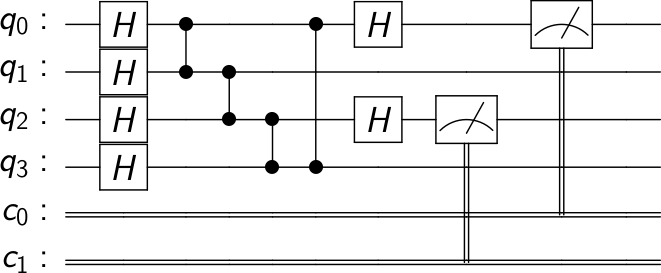
\includegraphics[scale=0.25]{circuit}
\end{figure}

\pause
Cluster state: \cite{jozsa}

\begin{figure}[!htb]
	%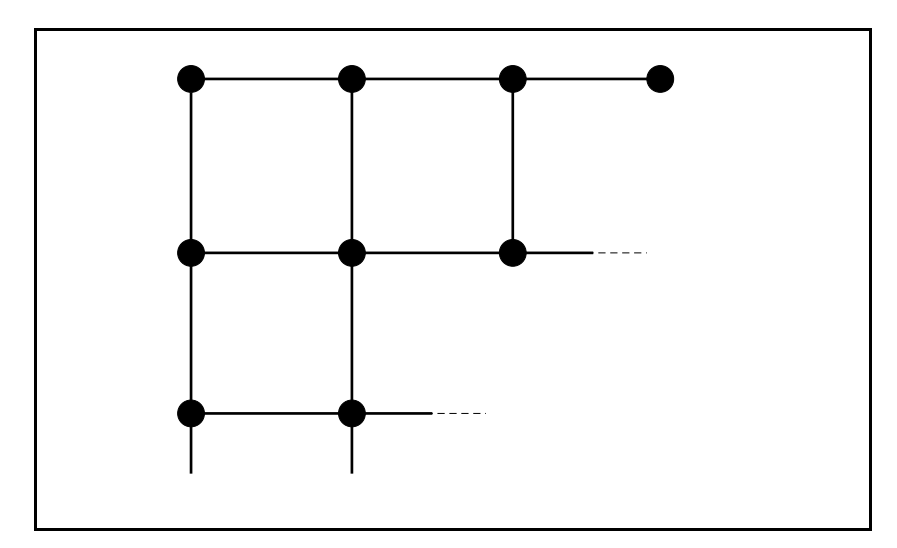
\includegraphics[scale=0.2]{jozsa1}
	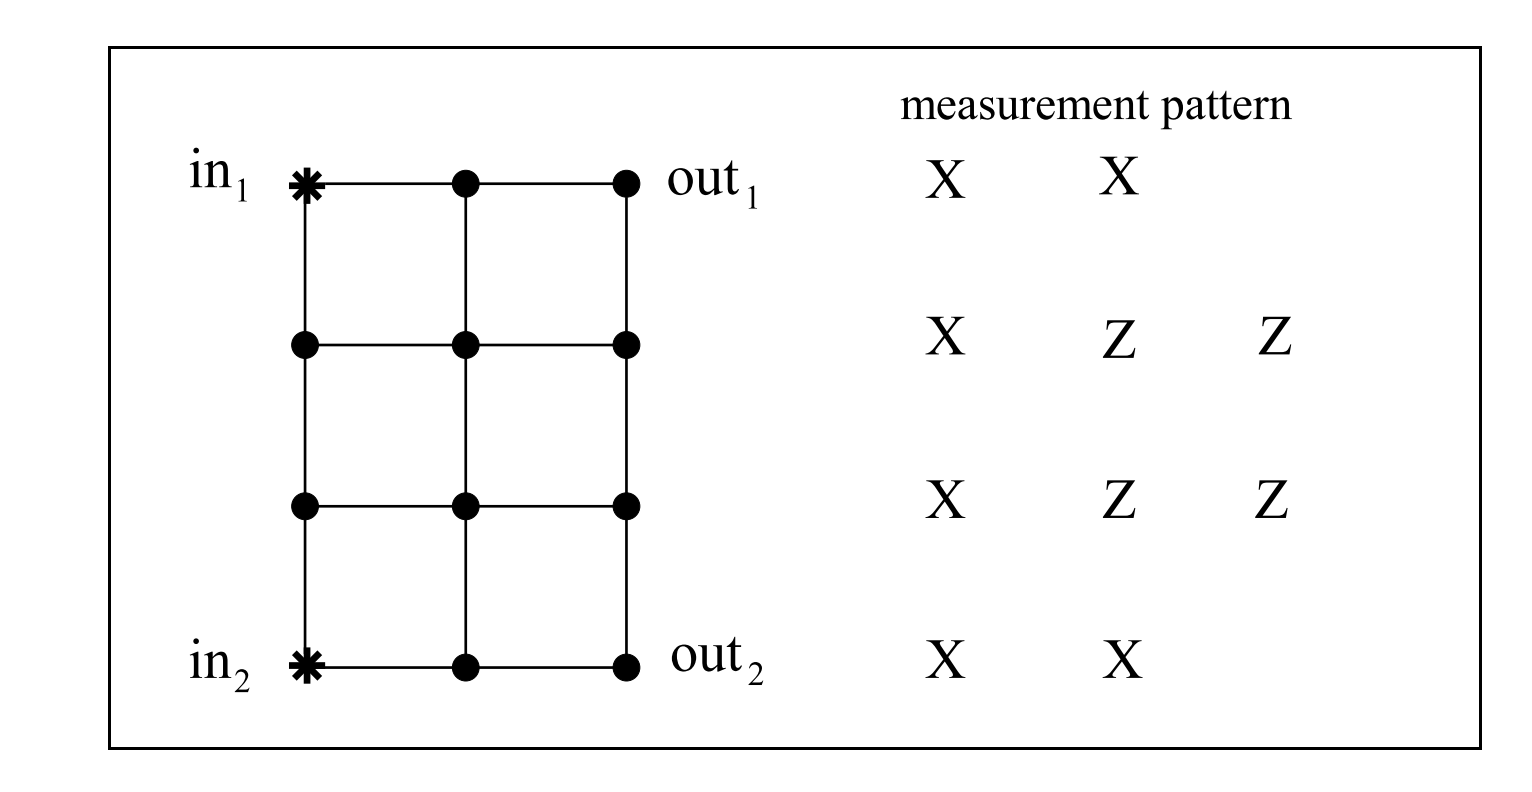
\includegraphics[scale=0.18]{fig8}
\end{figure}







\end{frame}


\begin{frame}[fragile]
\frametitle{MBQC: One-way quantum computer}
Quantum teleportation = Entanglement + Measurement

\begin{center}
	$\,$\Qcircuit @C=.7em @R=1.4em  {
		\lstick{\ket{\psi}} & \qw & \ctrl{1} & \gate{HZ_\theta} & \meter &  \\
		\lstick{\ket{+}}    & \qw & \ctrl{0} & \qw & \qw &\rstick{X^m H Z_\theta \ket{\psi}} 
	}
	
\end{center}

\pause

\begin{figure}[!htb]
	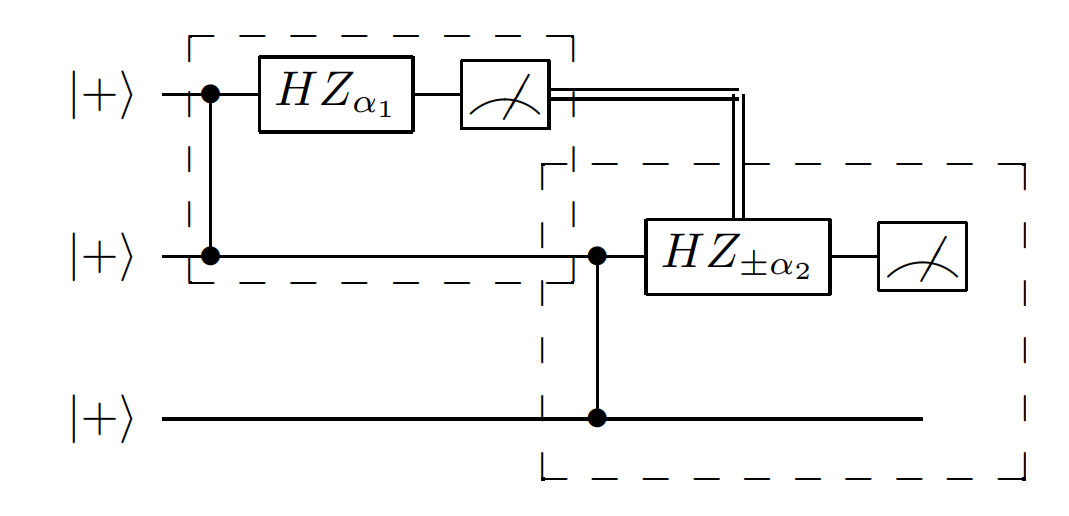
\includegraphics[scale=0.25]{cluster6}
	\caption{From \cite{nielsen}}
\end{figure}


\end{frame}


\begin{frame}
\frametitle{MBQC: One-way quantum computer}

Universality: Quantum circuit model $\equiv$ Cluster state formulation. \pause How? \pause

\begin{itemize}
	\item Transfer of information by teleportation
	\pause
	\item Any qubit rotation can be done on a chain of qubits
	\pause
	\item The CNOT gate can be implemented in a ``T'' configuration
\end{itemize}
\pause
\begin{figure}[!htb]
	\begin{subfigure}{.5\textwidth}
		\centering
		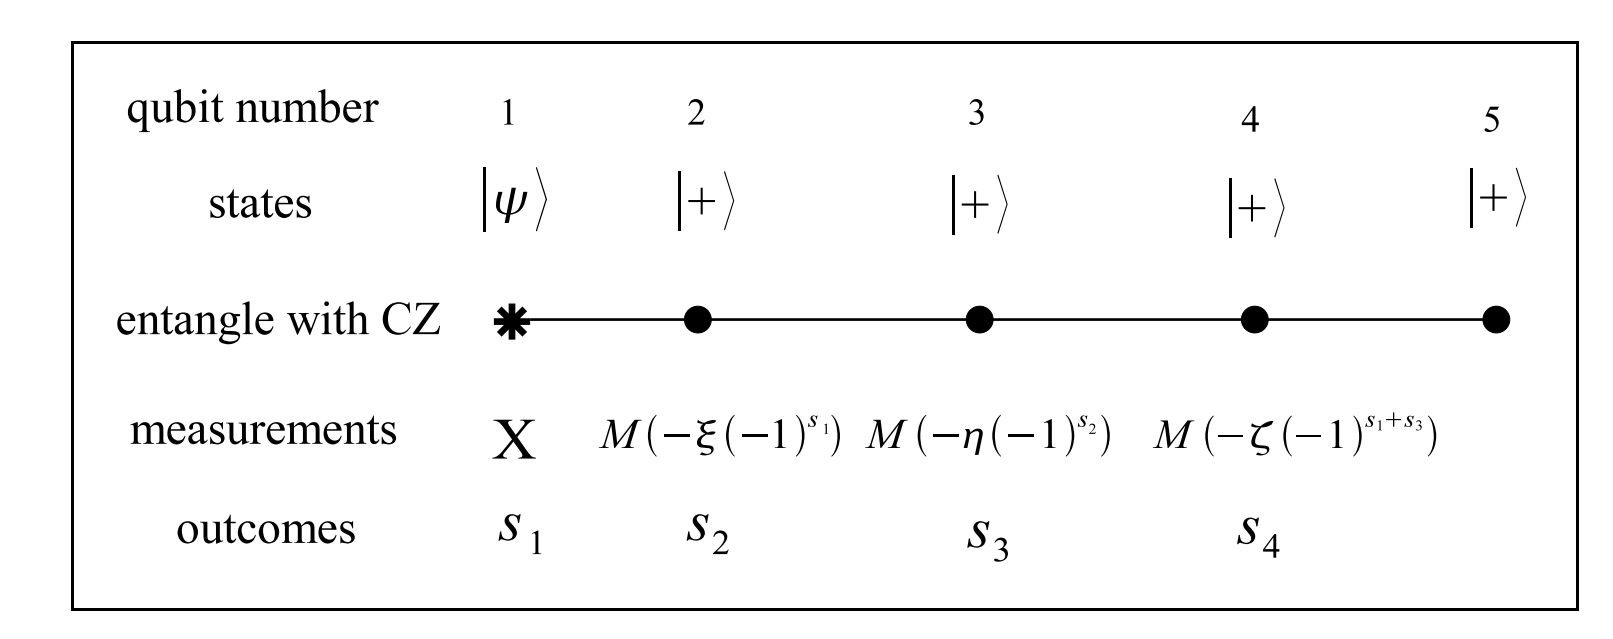
\includegraphics[scale=0.15]{rotate}
		\caption{From \cite{jozsa}}
	\end{subfigure}%
	\begin{subfigure}{.5\textwidth}
		\centering
		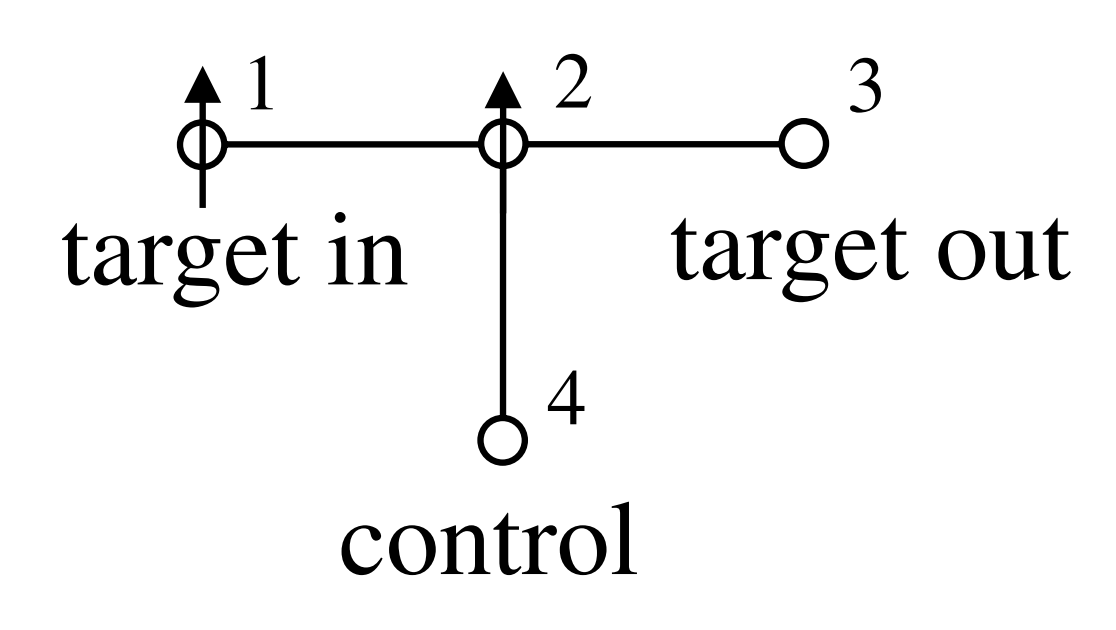
\includegraphics[scale=0.15]{CNOT}
		\caption{From \cite{MBQC}}
	\end{subfigure}
	
	
\end{figure}






\end{frame}
%%%%%%%%%%%%%%%%%%%%%%%%%%%%%%%%%%%%%%%%%%%%%%%%%%%%%%%%%%%%%%%%

\begin{frame}
\frametitle{Variational simulation of non-trivial quantum states}

QAOA \cite{QAOA}: Quantum approximate optimization algorithm

\pause

\begin{itemize}
	\item Principle: Quantum adiabatic theorem on $H = H_2 + H_1$

	\pause
	
	\item Variational ansatz (modified in (\ref{eq:QAOAmod}))
	\begin{equation}\label{eq:QAOA}
	\boxed{\ket{\psi(\bm{\gamma}, \bm{\beta})} = \underbrace{ \strut {e^{-i\gamma_p H_1}e^{-i\beta_p H_2}} \dots {e^{-i\gamma_2 H_1}e^{-i\beta_2 H_2}} {e^{-i\gamma_1 H_1}e^{-i\beta_1 H_2}}}_{ p \mbox{ layers}} \ket{\psi_1}}
	\end{equation}
	\begin{itemize}
		\item $(\bm\gamma,\bm\beta) = (\gamma_p,\dots, \gamma_1,\beta_p,\dots, \beta_1)$
		
		\item $\ket{\psi_1} = $ ground state of $H_1$ (easy to prepare)
	\end{itemize}

    \pause
	
	\item Cost function:
	\begin{equation*}
	\text{Overlap: } \abs{\braket{\psi_0}{\psi(\bm\gamma,\bm\beta)}}^2 ,\quad \text{or} \quad \text{Energy:} \bra{\psi(\bm\gamma,\bm\beta)}H\ket{\psi(\bm\gamma,\bm\beta)}.
	\end{equation*}
\end{itemize}


\end{frame}

%%%%%%%%%%%%%%%%%%%%%%%%%%%%%%%%%%%%%%%%%%%%%%%%%%%%%%%%%%%%%%%%


\begin{frame}
\frametitle{Variational simulation of non-trivial quantum states}

\underline{Example}: GHZ state $\sim \ket{0}^{\otimes L} + \ket{1}^{\otimes L} $ 
\begin{equation*}
H_{GHZ} = -\sum^L_{i=1}Z_i Z_{i+1} = \underbrace{-\sum^L_{i=1}Z_i Z_{i+1}}_{H_2} - 0\underbrace{\sum^L_{i=1}X_i}_{H_1}, \qquad \ket{GS_{H_1}} = \bigotimes^L_{i=1} \ket{+}
\end{equation*}

\pause

$\implies$ Perfect fidelity, $p \sim L/2$.

\begin{figure}[!htb]
	\centering
	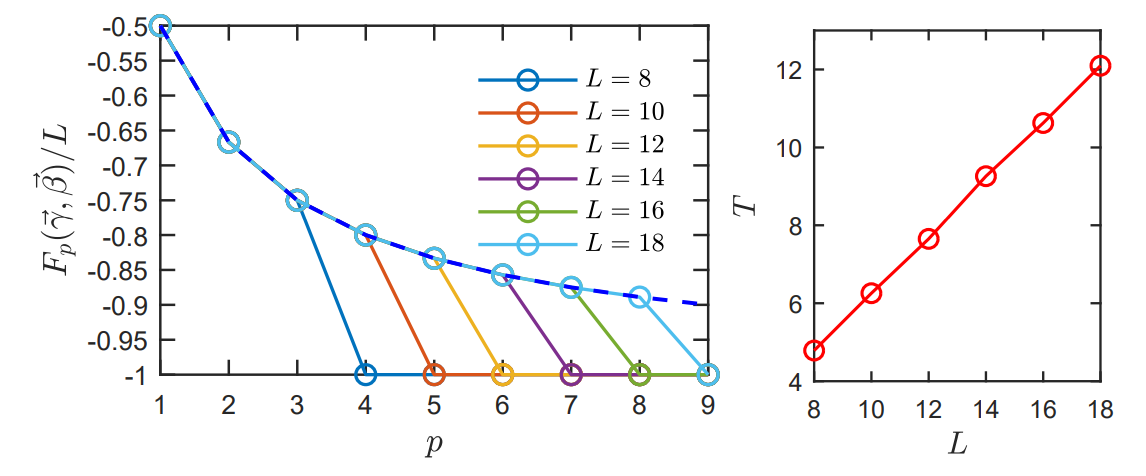
\includegraphics[scale=0.25]{ghz1}
	\caption{GHZ state simulation. Fidelity \& $p$ vs. $L$, \cite{VQCS}}
\end{figure}

\end{frame}


%%%%%%%%%%%%%%%%%%%%%%%%%%%%%%%%%%%%%%%%%%%%%%%%%%%%%%%%%%%%%%%%


\begin{frame}
\frametitle{Variational simulation of TFIM ground state}

\underline{Example}: Transverse field Ising model
\begin{equation*}
H \coloneqq H_2 + H_1 =  - \sum_{i=1}^L Z_i Z_{i+1} - g\sum^L_{i=i}X_i
\end{equation*}

\pause

$\implies$ Perfect fidelity, $p\sim L/2$
\begin{figure}[!htb]
	\centering
	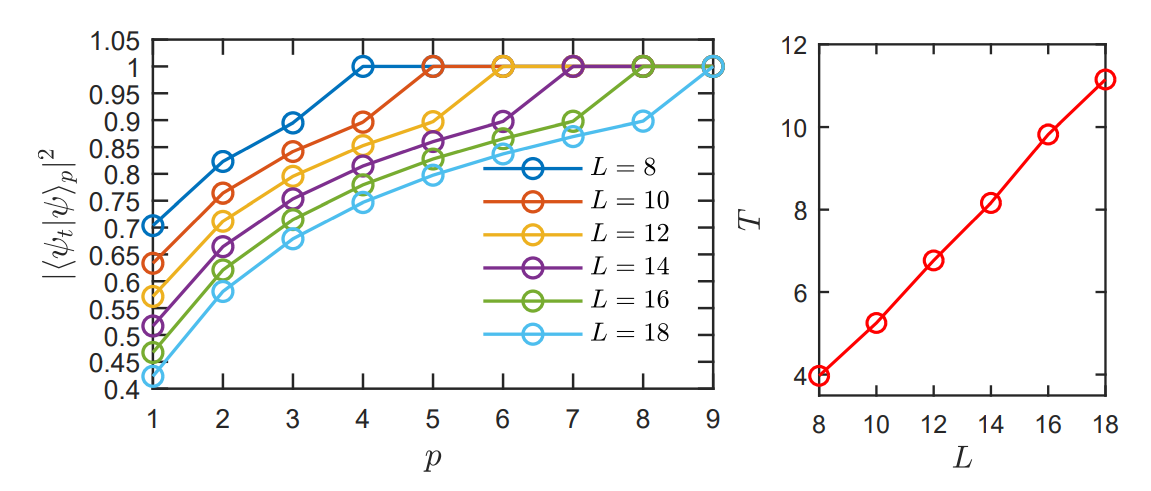
\includegraphics[scale=0.25]{tfim}
	\caption{TFIM state simulation. Fidelity \& $p$ vs. $L$, \cite{VQCS}}
\end{figure}






\end{frame}

%%%%%%%%%%%%%%%%%%%%%%%%%%%%%%%%%%%%%%%%%%%%%%%%%%%%%%%%%%%%%%%%

\begin{frame}
\frametitle{Variational simulation of TFIM ground state}


Limitations of protocol in \cite{VQCS}: 
\begin{itemize}
	
	\item Requires non-local unitaries. 
	
	\item  $p \sim L$.
	
	\item MERA construction \cite{MERA}: $p\sim \log(L)$, \\
	$\quad\quad\quad\quad\quad\quad\qquad\qquad$ but non-local unitaries required.
\end{itemize}

$\,$\\

\pause

$\implies$ Is a measurement-based QAOA scheme a solution?






\end{frame}





%%%%%%%%%%%%%%%%%%%%%%%%%%%%%%%%%%%%%%%%%%%%%%%%%%%%%%%%%%%%%%%%



\begin{frame}
\frametitle{Measurement-based QAOA for TFIM}

Hamiltonian
\begin{equation*}
H \coloneqq H_2 + H_1 =  - \sum_{i=1}^L Z_i Z_{i+1} - g\sum^L_{i=i}X_i
\end{equation*}


QAOA ansatz:
\begin{equation*}
\ket{\psi(\bm{\gamma}, \bm{\beta})} =  \strut {e^{-i\gamma_p H_1}e^{-i\beta_p H_2}} \dots {e^{-i\gamma_2 H_1}e^{-i\beta_2 H_2}} {e^{-i\gamma_1 H_1}e^{-i\beta_1 H_2}} \ket{\psi_1}
\end{equation*}

MBQC is universal $\implies$ Measurement-based QAOA ansatz is possible. \\

$\,$\\

Ingredients: $Z,X$-rotations, \& $CNOT$. \\

$\quad$ $\clubsuit$ Scheme can be simplified by changing measurement pattern.  






\end{frame}


%%%%%%%%%%%%%%%%%%%%%%%%%%%%%%%%%%%%%%%%%%%%%%%%%%%%%%%%%%%%%%%%


\begin{frame}
\frametitle{But...}
Limitations: 
\begin{itemize}
	\item $p \sim L$, where $p$ is the number of layers of measurements. 
	\item Non-local unitaries still required
\end{itemize}




$\,$\\
\pause
$\downarrow\downarrow\downarrow$\\

$\,$\\

Two possibilities:
\begin{itemize}
	\item QAOA is insufficient; need a completely new algorithm.
	\item QAOA is sufficient, but need better MBQC implementation. \pause $\impliedby$
\end{itemize} 



\end{frame}





%%%%%%%%%%%%%%%%%%%%%%%%%%%%%%%%%%%%%%%%%%%%%%%%%%%%%%%%%%%%%%%%

\begin{frame}
\frametitle{2nd possibility: How robust is QAOA?}

Test QAOA with TFIM without translation invariance:

\begin{equation}\label{eq:QAOAmod}
\mathcal{H} = \sum_{j} Z_j Z_{j+1} + \sum_j g_j  X_j
\end{equation}

\pause

Modified QAOA ansatz (reference (\ref{eq:QAOA}))
\begin{itemize}
	\item $p$ layers
	\item Each layer is parameterized by $(\bm\gamma,\bm\beta)_k = (\gamma_{1},\dots,\gamma_{L},\beta_{1},\dots,\beta_{L} )_k$.
\end{itemize}

\pause

\begin{conjecture}
	This modified QAOA can target the critical ground state with perfect fidelity for $p = L/2$. In which case, the total number of parameters is $L^2$.  
\end{conjecture}




\end{frame}


%%%%%%%%%%%%%%%%%%%%%%%%%%%%%%%%%%%%%%%%%%%%%%%%%%%%%%%%%%%%%%%%


\begin{frame}
\frametitle{2nd possibility: How robust is QAOA?}



Conjecture holds for small $N = 4, 6, 8, 10$, even at lower $p$:



\begin{figure}[!htb]
	\centering
	\begin{subfigure}{0.5 \textwidth}
		\centering
		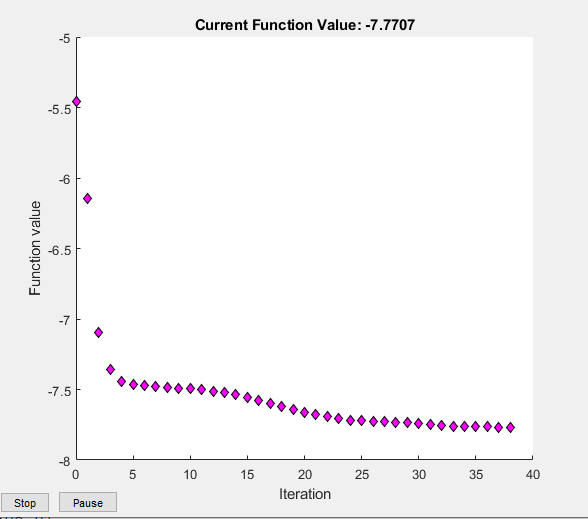
\includegraphics[scale=0.35]{N_6_p_3.PNG}
		\caption{$N=6$, $p=3$}
	\end{subfigure}%
	\begin{subfigure}{0.5 \textwidth}
		\centering
		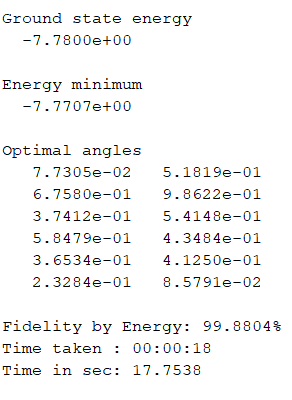
\includegraphics[scale=0.46]{N_6_p_3_out}
		\caption{99.9\% fidelity at low iteration count.}
	\end{subfigure}
\end{figure}

\end{frame}


%%%%%%%%%%%%%%%%%%%%%%%%%%%%%%%%%%%%%%%%%%%%%%%%%%%%%%%%%%%%%%%%

\begin{frame}
\frametitle{2nd possibility: How robust is QAOA?}


(Using the overlap as the cost function in this case)



\begin{figure}[!htb]
	\centering
	\begin{subfigure}{0.5 \textwidth}
		\centering
		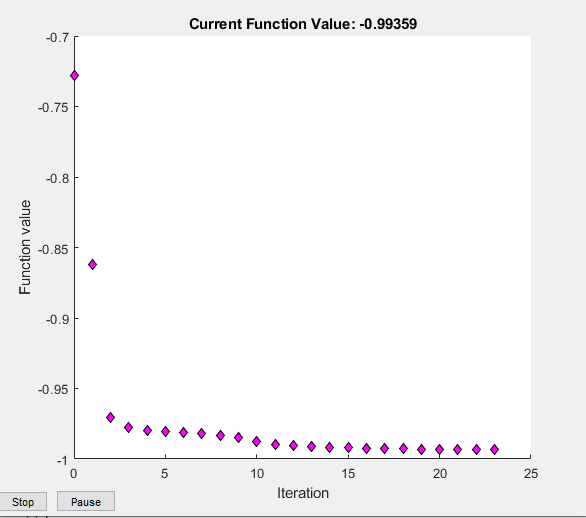
\includegraphics[scale=0.35]{N_8_p_4.PNG}
		\caption{$N=8$, $p=4$}
	\end{subfigure}%
	\begin{subfigure}{0.5 \textwidth}
		\centering
		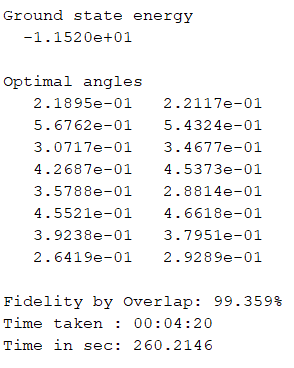
\includegraphics[scale=0.46]{N_8_p_4_out}
		\caption{99.4\% fidelity at low iteration count.}
	\end{subfigure}
\end{figure}

\end{frame}



%%%%%%%%%%%%%%%%%%%%%%%%%%%%%%%%%%%%%%%%%%%%%%%%%%%%%%%%%%%%%%%%


\begin{frame}
\frametitle{2nd possibility: How robust is QAOA?}





\begin{figure}[!htb]
	\centering
	\begin{subfigure}{0.5 \textwidth}
		\centering
		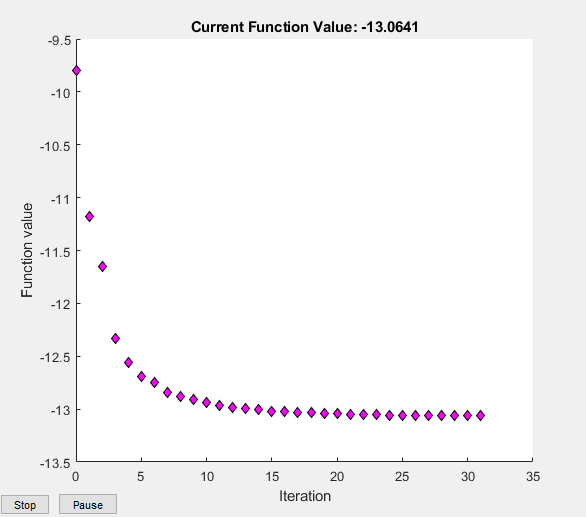
\includegraphics[scale=0.30]{N_10_p_2.PNG}
		\caption{$N=10$, $p=2$ only}
	\end{subfigure}%
	\begin{subfigure}{0.5 \textwidth}
		\centering
		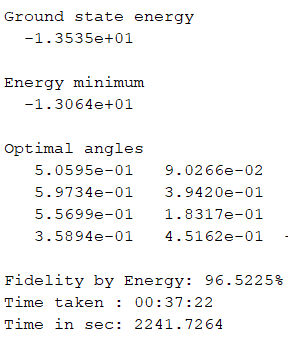
\includegraphics[scale=0.47]{N_10_p_2_out}
		\caption{96\% fidelity, not bad for $p=2$.}
	\end{subfigure}
\end{figure}

\pause

$\implies$ Small $N$ due to large parameter space ($\sim L^2$) and limitations in computing power and algorithm efficiency.











\end{frame}




%%%%%%%%%%%%%%%%%%%%%%%%%%%%%%%%%%%%%%%%%%%%%%%%%%%%%%%%%%%%%%%%


\begin{frame}
\frametitle{Summary}


\begin{itemize}
	\item MBQC
	\item Variational non-trivial state simulation \& QAOA
	\item Measurement-based QAOA. It is a good idea?
	\item Robustness of QAOA, tested on TFIM with non-constant $g_i$.
	
	\pause
	
	\item \textbf{Next?} Jordan-Wigner transform $\implies$ Reduce problem size 
\end{itemize}


\end{frame}


%%%%%%%%%%%%%%%%%%%%%%%%%%%%%%%%%%%%%%%%%%%%%%%%%%%%%%%%%%%%%%%%


\begin{frame}[allowframebreaks]
\frametitle{References}



\bibliographystyle{amsalpha}
\bibliography{references}{}



\end{frame}










\end{document}